\chapter{802.11 Wireless Standards}

Currently there are a lot of 802.11 standards. The important ones are listed
in the table~\ref{tab:802.11ws:list}

\begin{table}[t]
\centering
\resizebox{\textwidth}{!}{%
\begin{tabular}{|l|p{10cm}|}
\hline
\textbf{802.11 Typology} & \textbf{Description}                                                     \\ \hline
802.11a                  & 54Mb/s, 5GHz. Launched in 2001, took more to develop than "b"            \\ \hline
802.11b                  & 5.5/11Mb/s. Launched in 1999, it was the first 802.11 protocol ever made \\ \hline
802.11e                  & It brings QoS (Quality of Service) extension                             \\ \hline
802.11g                  & 54Mb/s, 2.4GHz, compatible with "b"                                      \\ \hline
802.11n                  & High throughput technology - introduces MIMO                             \\ \hline
802.11p                  & It brings communication between vehicles but also for payments           \\ \hline
802.11s                  & It brings extension for mesh networks                                    \\ \hline
\end{tabular}%
}
\caption{List of most important 802.11 wireless standards}
\label{tab:802.11ws:list}
\end{table}

\section{802.11e}

802.11e as already said brings QoS (quality of service) extension. This doesn't
mean you'll always have a good quality of service.
802.11 used initially two type of ways to challenge data: \textbf{DCF}
(distributed coordination function) and \textbf{PCF} (point coordination
function). From these two methods, \textbf{HCCA} was created.

\paragraph*{DCF} This is the basic access method for 802.11, and offers CSMA/CA
for transmitting in the channel.

\paragraph*{PCF}\todo{This paragraph is very confused, please check it out
  carefully!} It's a priority that is centrally controlled,\todo{I've copied
  what's been written in the slides, but I dunno what it means!} the PC (point
coordinator) is usually also the AP (access point).
After each beacon there is a CP (content period) and a CFP (contention free
period). PCF has several problems that lead this channel access method to not
being used in practice, also because there is no mechanism to preserve bandwidth
or characterize traffic in any way.

\paragraph*{HCCA} It's a DCF inspired system, created as an extension of PCF,
and it uses contention free periods. In contrast to PCF, in which the interval
between two beacon frames is divided into ten periods of CFP and CP, the HCCA
allows for CFPs being initiated at almost anytime during a CP. In this case,
CFP is called CAP. During the CP, all stations function in EDCA mode, instead
during CAP, the hybrid coordinator (the AP) controls the access to the medium.
HCCA has the following characteristics:
\begin{itemize}
\item Efficient use of bandwidth
\item Guarantees latency and bandwidth
\item Has a complex scheduler and added complexity
\end{itemize}

This way to challenge data is optional, and it's not implemented to any
significant level.\\[5pt]


\noindent Additionally, 802.11 provides two types of contention window:
\textbf{normal} and
\textbf{adaptive}.

\paragraph*{Normal contention window} This type of contention window select a
random number from a range that goes from 0 to $cw$\todo{I don't understand
  from where this $cw$ came out :/}. The size of $cw$ is small, ensuring less
wastage of idle slots time but causing a large number of collisions with
multiple senders (two or more station can reach zero at once).

\paragraph*{Adaptive contention window} The adaptive contention window starts
with $cw = 31$ and when no CTS or ACK are received from a communication it then
sets the cw to $2 \cdot cw + 1$\footnote{So it'll become $63, 127, 255$.}.
Finally, when the transmission succeed, the $cw$ will be reset to $31$.
The adaptive scheme is unfair, and under contention, unlucky nodes will use
larger $cw$ than luckier one (due straight reset after a success). Having larger
$cw$ means that while unlucky nodes are counting down for access to the channel
lucky nodes may be able to transmit several packets. 802.11 adaptive contention
window doesn't provide QoS.

\subsection{EDCA}

EDCA is a supported QoS mechanism in 802.11e. It has four access categories:
\begin{enumerate}
\item AC\_V0 (for voice) $\to$ when you want to be fast but you leave the
  channel soon. it's privileged to the others, especially during congestion.
  It has a small $cw_{max}$ (7) because otherwise you'll end up with collisions.
\item AC\_V1 (for video)
\item AC\_BE (best effort) $\to$ the difference is present only on the
  initiation phase
\item AC\_BK (background) $\to$ with this access category, you don't care to be
  fast
\end{enumerate}

EDCA has 8 traffic classes (TC) too.
Each AC starts a back off after detecting the channel being idle for AIFS, and
after waiting for it, each back off sets counters choosing between $1$ and
$cw + 1$. The back off formula is:
\begin{equation}
newCW[AC] \ge ((oldCW[TC] + 1) \cdot PF) - 1
\end{equation}

The MSDU (Max Service Data Unit) are delivered through multiple back offs
within one station using AC specific parameters.

With EDCA video streams capacity drops. With more collisions I have larger
contention windows, and with multiple streams I lose some overall bandwidth.

\paragraph*{Prioritized channels} Similar to DCF, but with four priorities, EDCA
offers prioritized channel, based on the QoS parameters per traffic classes,
which includes:
\begin{itemize}
\item AIFS[AC]\footnote{AIFS means \textit{Arbitration Inter-frame space}}
\item CWmin[AC]
\item PF[AC]\footnote{PF means \textit{Persistence Factor}}
\end{itemize}

\subsubsection{Pro and Cons}

Using EDCA has the following advantages:
\begin{itemize}
\item Voice and video have priority over data
\item It works well with a slightly loaded network
\end{itemize}
but has the following disadvantages:
\begin{itemize}
\item Streams of the same priority compete: making difficult for ECDA to be able
  to guarantee a good access, latency, bandwidth or jitter to every connection.
A solution to this problem is using \textbf{admission control}.
\end{itemize}

\paragraph*{Admission Control} This solution allows only a limited number of
peers to access the network, limiting (but not eliminating) the stream
contention and reducing the latency of QoS streams.
In this way the best-effort approach is no more necessary.
\subparagraph*{How Admission Control works} The AP advertises ACM\footnote{This
is a bit that says if the AP supports Admission Control.} in beacon to indicate
if admission control is mandatory for any Access Category. In this way, to use
and AC that  sends AddTS (\textit{Add Traffic Specification}) Request Action
Frame to AP that includes a TSPEC.
When a new node wants to connect with the AP, the AP runs the admission control
algorithm and replies with an AddTS Response Action Frame.

\section{802.11n}

This version supports legacy mode (a/b/g), and offers more bandwidth for QoS
applications, a greater wireless range and throughput.
The high data rates sometimes can cause interference with radar signals,
typically with 2 transmitters MIMO the data rate can go up 300Mbps (on a 40MHz
channel).

\subsection{802.11n enhancements}

This 802.11 version brings different enhancements.

\paragraph*{MAC layer} at the MAC layer there are the following benefits:
\begin{itemize}
\item Smaller packets
\item Combine ACK for more packets
\item Packets aggregation
\end{itemize}

\paragraph*{Physical layer} At the physical layer, both for 2.4GHz and 5GHz we
have:
\begin{itemize}
\item Smaller slots
\item Better modulation (OFDM)
\item MIMO (\textit{Multiple Input Multiple Output}) radio technology with
spatial multiplexing $\to$ transmit and receive with multiple radios
simultaneously in some spectrum. MIMO is useful because one antenna can break
but the communication would still be possible, thing that would not be possible
with SISO (\textit{Single Input Single Output}), that, on the other hand, has a
lower-cost and has a simpler implementation than MIMO\footnote{
SISO has this additional disadvantages though:
\begin{itemize}
\item the energy is wasted sending in all directions
\item it's sensitive to interference from all directions
\end{itemize}
}. At the end of the day, MIMO presents the following advantages:
\begin{itemize}
 \item the signal has more power
 \item transmits twice the amount of data
\end{itemize}
\end{itemize}

\section{802.11p}

This protocols is designed to provide connectivity to vehicles. Since it's
still under heavy development it's not freely available at the moment.
Governments have reserved particular channel, 5.9GHz in USA and EU. 802.11p
allows up to 300m communication range with 6Mbps. Transfers are possible
even at 200km/h.

This wireless version uses DCF schema with a different period. A lot of
research is going on in particular about routing schemes and MAC layers.

\subsection{802.11p applications}

The mayor application for this wireless standard is \textbf{safe driving}.
When an incident is detected, alert messages are sent from the Abnormal
Vehicle\footnote{AV is a vehicle that its behavior is not conform to some
threshold}\todo{This footnote needs a rewrite} to the following vehicles, via
broadcast. This messages are faster than the normal human reaction, and can
prevent chained car accidents. How much time does it take to the following
vehicles to receive the message to break? The latency it's an important aspect.
Broadcasting messages could lead to an explosion when we have multi-hop path.
To solve this, different solutions have been proposed.
First of all, all the cars needs to have locations, so they can include details
when they send the ``emergency message'', such as:
\begin{AutoMultiColItemize}
\item geographical location
\item speed
\item acceleration
\item moving direction
\end{AutoMultiColItemize}

\begin{figure}[t]
  \centering
  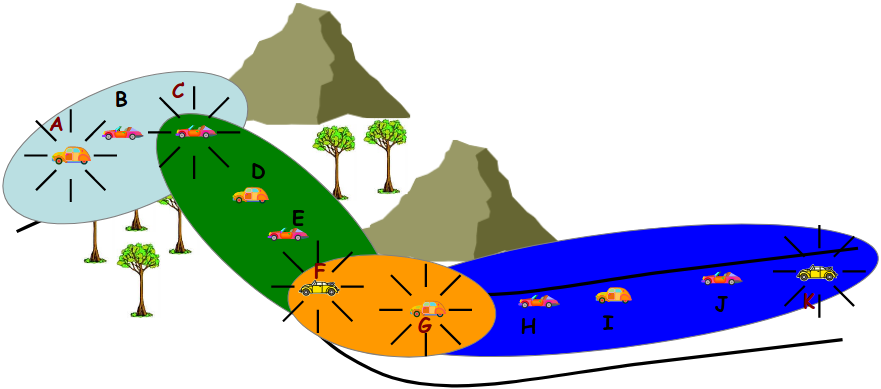
\includegraphics[scale=0.4]{broadcast}
  \caption[Optimal broadcast example]{
    An example of an optimal broadcast: A, C, F, G and F broadcast the alert
    message, meanwhile the other cars receive the message but don't send it
    again, thus reducing the overall interference.
  }
  \label{fig:802.11ws:broadcast}
\end{figure}

The car movement needs to be kept in consideration: cars can move very fast,
causing variable transmission range. On top of that, a car cannot be sure to
be the farthest car receiving that broadcast message, as explained in
Figure~\ref{fig:802.11ws:broadcast}. So who has to forward the alert message?
It's important to pick up the right vehicle that has to propagate the message.
If the message has already been rebroadcast by a following vehicle do not
forward it, because it could be redundant. A way to reduce the message
retransmission is to use a sort of back-off mechanism, or otherwise set vehicles
contention window with an inverse proportion of the distance from the sender,
but it has the unrealistic assumption that there is an unique, constant, and
known-a-priori transmission range.

\subsubsection{Using minimum connect dominating set} The MCDS identify the
minimum number of sets that allows you to cover the whole set\footnote{A minimum
  connected dominating set of a graph G is a connected dominating set with the
  smallest possible cardinality among all connected dominating sets of G. The
  connected domination number of G is the number of vertices in the minimum
  connected dominating set. See more at
  \url{https://en.wikipedia.org/wiki/Connected_dominating_set}.
}.
Although it seems a good solution for this problem, it has the following
issues:
\begin{itemize}
\item only the one in the MCDS can propagate the message, making the solution
  optimal, but not feasible: I would need a central station then knows all the
  other nodes position
\item this solution is not considering the number of hop of a message has to
  traverse
\end{itemize}

\subsubsection{Urban multi-hop broadcasting protocols} This broadcasting
protocols uses \textbf{jamming} signals to determine the next forwarder:
vehicles receiving an alert message emit a jamming signal for a time that's
proportional to the distance from the sender. The last one stops the hamming
signal and forward the message.

The problem of this solution is that is slow, and for this is not suitable for
alert messages (jamming signal phase delays the transmission of the message).

\subsubsection{Fast Broadcast}
Fast broadcast is designed to have Alert Messages covering the area of interest
in less time possible. It uses two type of packets: \textit{Hello messages} and
\textit{Alert messages}. Hello messages contain the sender's position and the
maximum forward distance from which another vehicle has been heard transmitting
another hello message. In particular it contains:
\begin{itemize}
\item CMBR (\textit{Current Maximum Backward Range}): the maximum backward
  distance at which some car would be able to hear me
\item CMFR (\textit{Current Frontward Range}): the maximum distance from which
  I have been able to hear another car in front of me
\end{itemize}

Fast Broadcast has two phases:
\begin{enumerate}
\item estimation of transmission range between two vehicles (called
  \textit{hello messages}). This phase has little overhead and it's divided in
  rounds: at every round
  hello messages are randomly sent
\item transmission is used during broadcasting to reduce message number of hops
  (\textit{alert messages}\footnote{This message includes the estimated
  transmission range for that hop.})
\end{enumerate}

\begin{figure}
  \centering
  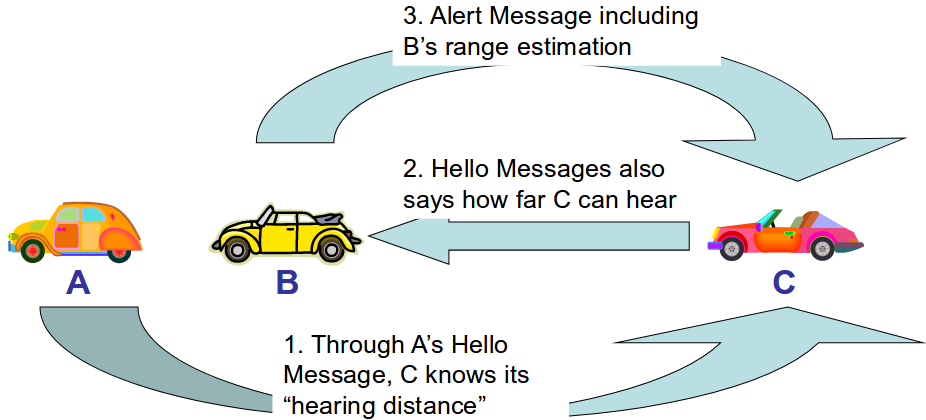
\includegraphics[scale=0.35]{fastBroadcast}
  \caption[Hello Message propagation]{A little illustration of how hello
    messages are delivered through the cars.}
  \label{fig:802.11ws:helloMessageDelivery}
\end{figure}

When a car receives a message, as illustrated in
Figure~\ref{fig:802.11ws:helloMessageDelivery}, it can be from two directions:
in front of it (and in that case it's an update), or behind it (and in that case
you update your transmission range).

The characteristics of this multi-hop broadcast protocol for vehicular networks
are:
\begin{itemize}
\item estimation of the maximum transmission range with few hello messages
\item minimization of the number of hops to be traversed
\item reduction of the delivery time
\end{itemize}

\paragraph*{Handling an AV} When an Abnormal Vehicle (AV) occurs, an alert
message is generated, and received by the nearby cars. The cars that received
the message wait a time that is proportional to the node's position with
respect to the estimated maximum transmission range. In particular, farthest
nodes transmit before the others: if another car that is farther from the source
has already forwarded the alter message, then the considered car abort its
sending procedure (since the message has already been propagated). The
contention window during this procedure is calculated in this way:
\begin{equation}
\left [ \left ( \frac{MaxRange - Distance}{MaxRange} \cdot (CW_{max} - CW_{min}) \right ) + CW_{min} \right ]
\end{equation}

\paragraph*{Comparing Fast Broadcast}
Let's compare Fast Broadcast with Static 300 and Static 100. Static 300 has a
lot of collision for 1 km of transmission range, determining Fast Broadcast as
the best solution. Static 100 performance are in general very poor.

\begin{figure}[t]
  \centering
  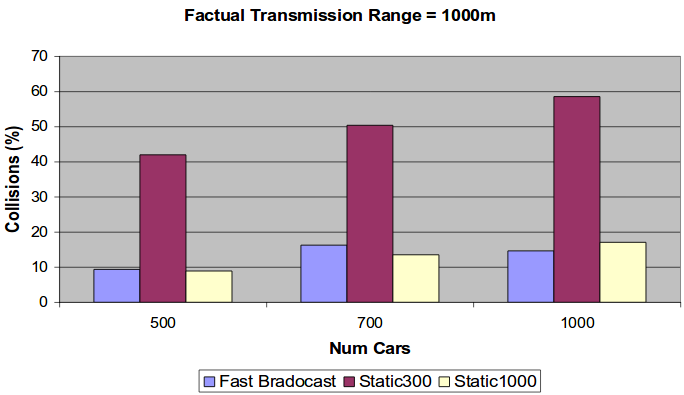
\includegraphics[scale=0.5]{fastBroadcastCollisionComparison}
  \caption[Fast broadcast comparison]{This histogram illustrates a comparison
    between Fast Broadcast, Static 300 and Static 100 over 1000m of actual
    transmission range: how is possible to see, the number of collision is very
    high for Static 300 at this distance, while Fast Broadcast and Static 100
    have similar results.}
  \label{fig:802.11ws:fastBroadCastComparison}
\end{figure}

These results are due the fixed nature of the contention window of Static 300
and Static 100, that after a certain distance start to have the same contention
contention window for farther cars. With small contention windows there is a
surge of collisions.
